\chapter{Result and Discussion}

\section{Introduction}
In this chapter, the result of signal identification will be displayed and explained. Furthermore, the result of the measurement system which includes the schematic of the system will be shown. After that, the vehicle simulation program and the result of 1 lap of simulation around Sepang North Track will be displayed and discussed. Finally, several strategies planned using the simulation software will be shown follow by discussion on which strategy is better and comparison between the strategies.

\section{Signal Identification}

\section{Measurement System}

\section{Vehicle Simulation}
The vehicle dynamics simulation software is built. As explained in last chapter, the simulation software has the ability to simulate the vehicle behaviour when driving around the Sepang North Track. As shown in figure \ref{im:vehicleSettings}, the software is initialized before the simulation can be started. The software takes a few parameter for initialization of the vehicle model which includes the vehicle driving wheel diameter, the total mass of the electric vehicle include the mass of the driver, the frontal area of the electric vehicle, the coefficient of rolling resistance and the coefficient of drag. The parameter for initializing the vehicle model is shown in table \ref{tb:vehicleModelParameter}.

\begin{figure}[htb]
	\centering
	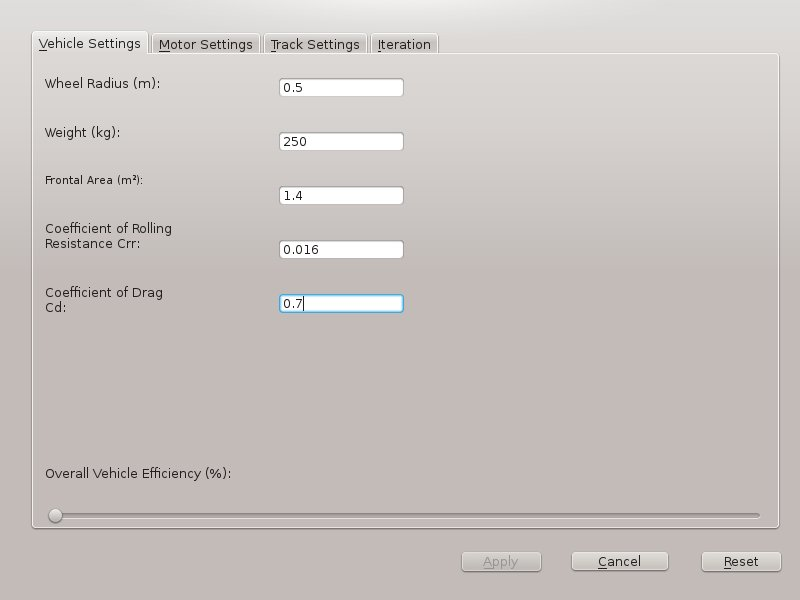
\includegraphics[width=5in]{images/vehicle_settings.jpg}
	\caption{Vehicle parameter for initializing the vehicle model}
	\label{im:vehicleSettings}
\end{figure}

\begin{table}[htbp]
\begin{center}
\begin{tabular}{|c|c|}
\hline
\textbf{Parameter} & \textbf{Value} \\ \hline
Wheel Radius & 0.5 m \\ \hline
Total Vehicle Mass & 250 kg \\ \hline
Frontal Area & 1.4 $m^2$ \\ \hline
Crr & 0.016 \\ \hline
Cd & 0.7 \\ \hline
\end{tabular}
\end{center}
\caption{Parameters for building the electric vehicle model}
\label{tb:vehicleModelParameter}
\end{table}

The motor and track model is initialized at the second and third tab of the initialization dialog as shown if figure \ref{im:motorSettings} and figure \ref{im:trackSettings}. At the last tab, the displacement interval for iteration is set which has a range from 1m to 25m, which is shown in figure \ref{im:iterationStep}.

\begin{figure}[htb]
	\centering
	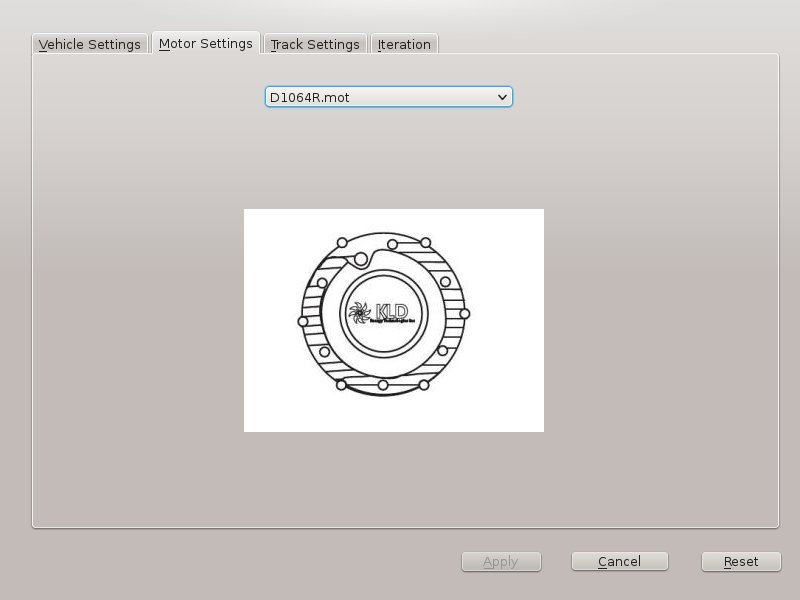
\includegraphics[width=5in]{images/motor_settings.jpg}
	\caption{Choosing the motor model}
	\label{im:motorSettings}
\end{figure}

\begin{figure}[htb]
	\centering
	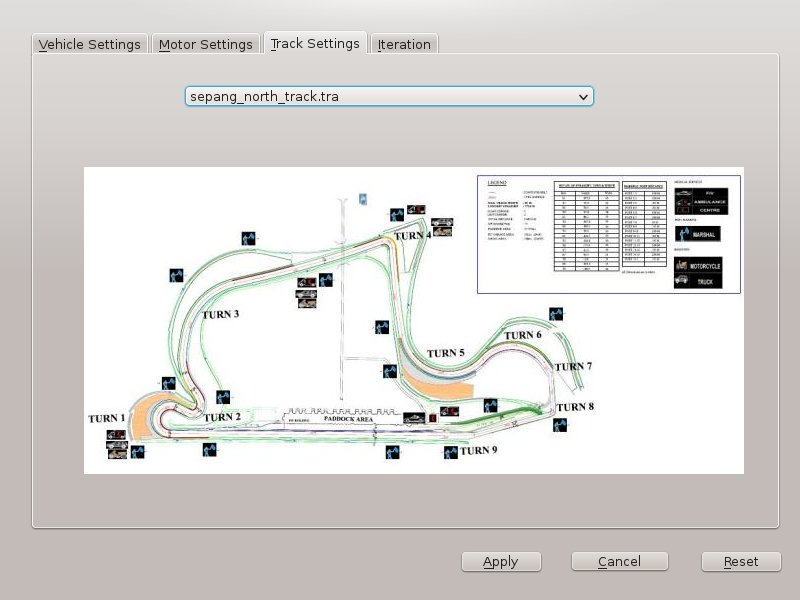
\includegraphics[width=5in]{images/track_settings.jpg}
	\caption{Choosing the track model}
	\label{im:trackSettings}
\end{figure}

\begin{figure}[htb]
	\centering
	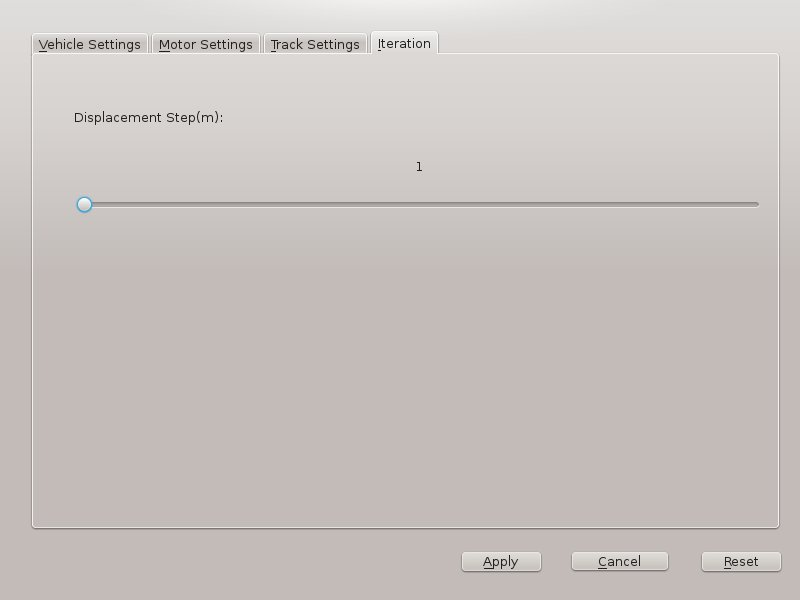
\includegraphics[width=5in]{images/iteration_step.jpg}
	\caption{Setting the displacement interval for iteration}
	\label{im:iterationStep}
\end{figure}

The simulation was run using "full throttle everywhere" strategy. The "full throttle everywhere" is the fundamental strategy for building the baseline data by applying full throttle over the entire circuit, which would give a maximum energy consumption result. The graph listed below is plot based on the simulation result:

\begin{itemize}
	\item{Speed and gradient versus displacement}
	\item{Power and gradient versus displacement}
	\item{Air drag versus displacement}
\end{itemize}

The graph of vehicle speed and track gradient versus the displacement is shown in figure \ref{im:0_1}. According to the graph, the maximum speed is 20.6m/s. The maximum speed is achieved at 1100m where the vehicle is driving downhill. The speed of the vehicle fluctuates between 20.6m/s and 12.6m/s from 1100m displacement onwards until end of the lap. The vehicle speed varies with the pattern of the gradient which it slows down when going up the hill because the torque generated is less than the total resistance torque excerted on the vehicle. The electric vehicle speeds up when going down the hill simply because the torque generated is excessive.

\begin{figure}[htb]
	\centering
	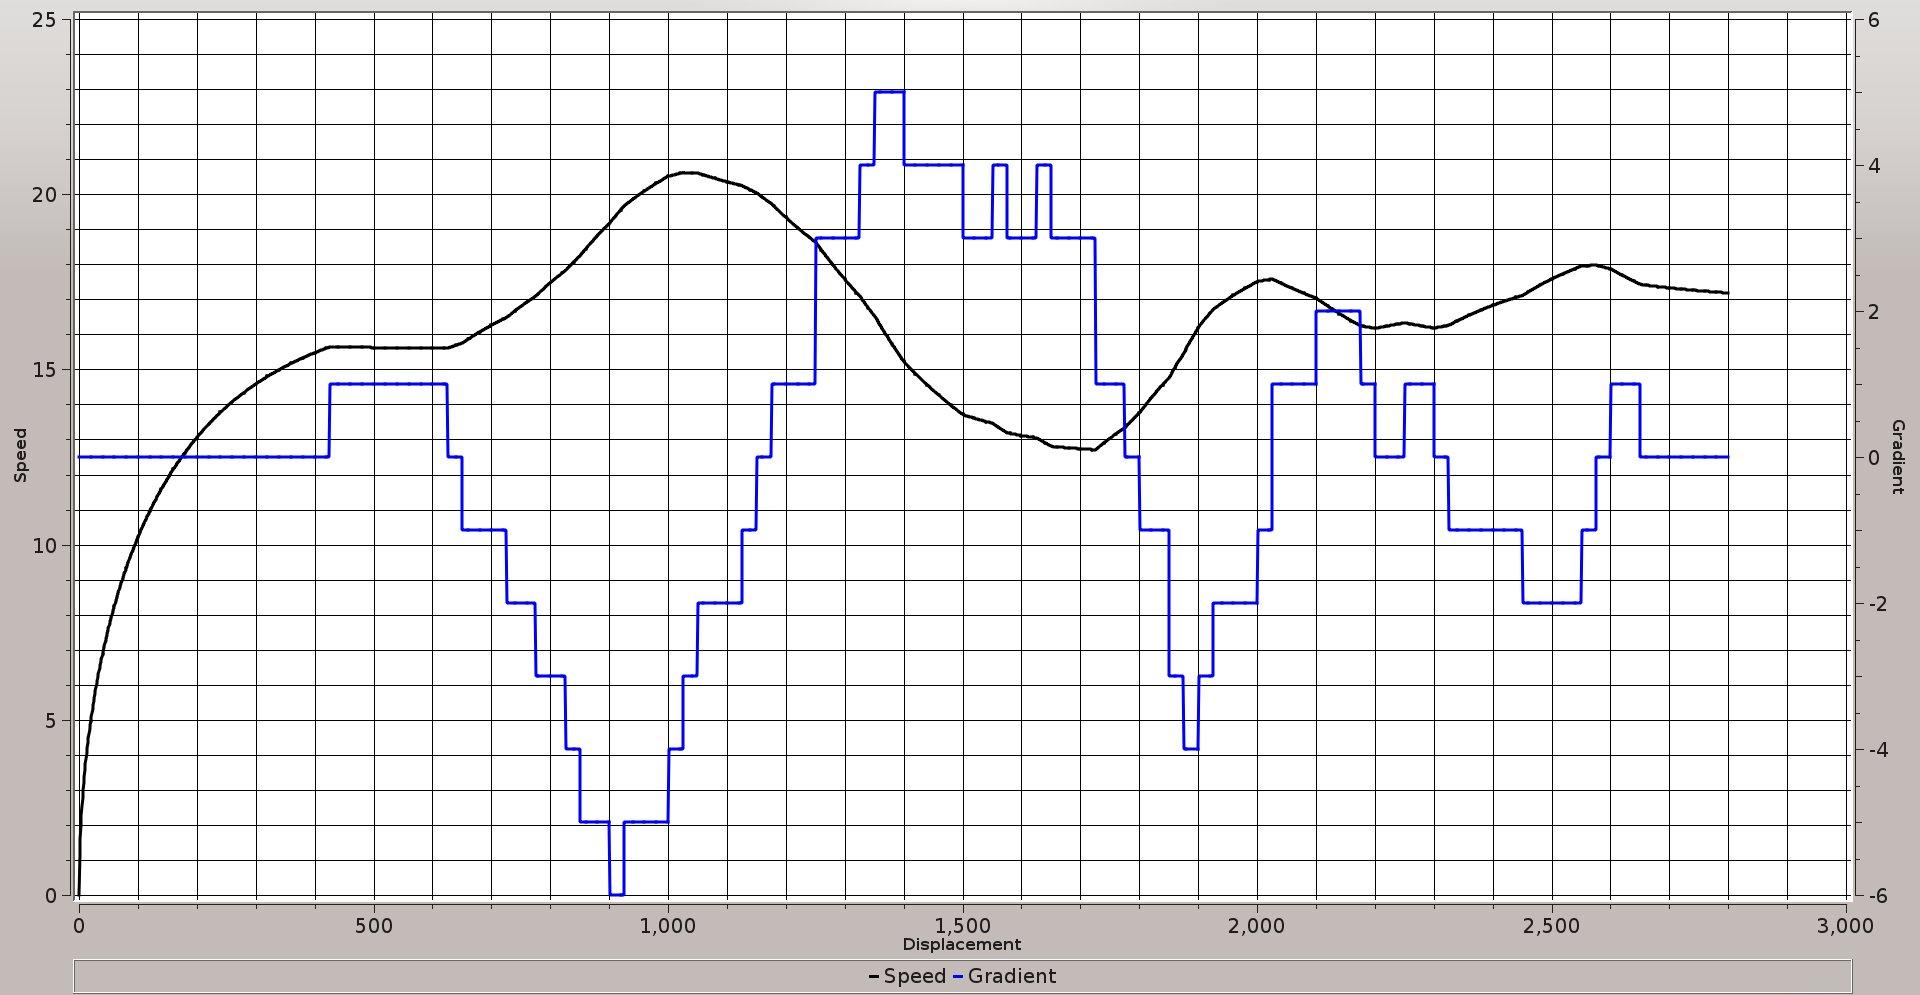
\includegraphics[width=6in]{images/0_1.jpg}
	\caption{Graph of speed and gradient versus displacement for "full throttle everywhere"}
	\label{im:0_1}
\end{figure}

Figure \ref{im:0_2} shows the power and gradient versus displacement. The power profile is the same as the speed profile as the torque generated by the electric motor is the same throughout the whole circuit which is constant 100N.m output. This is because the maximum torque output of the motor below 800RPM is 100N.m. The maximum power output of the electric vehicle is at around 1000m with a value of 4050W. 

\begin{figure}[htb]
	\centering
	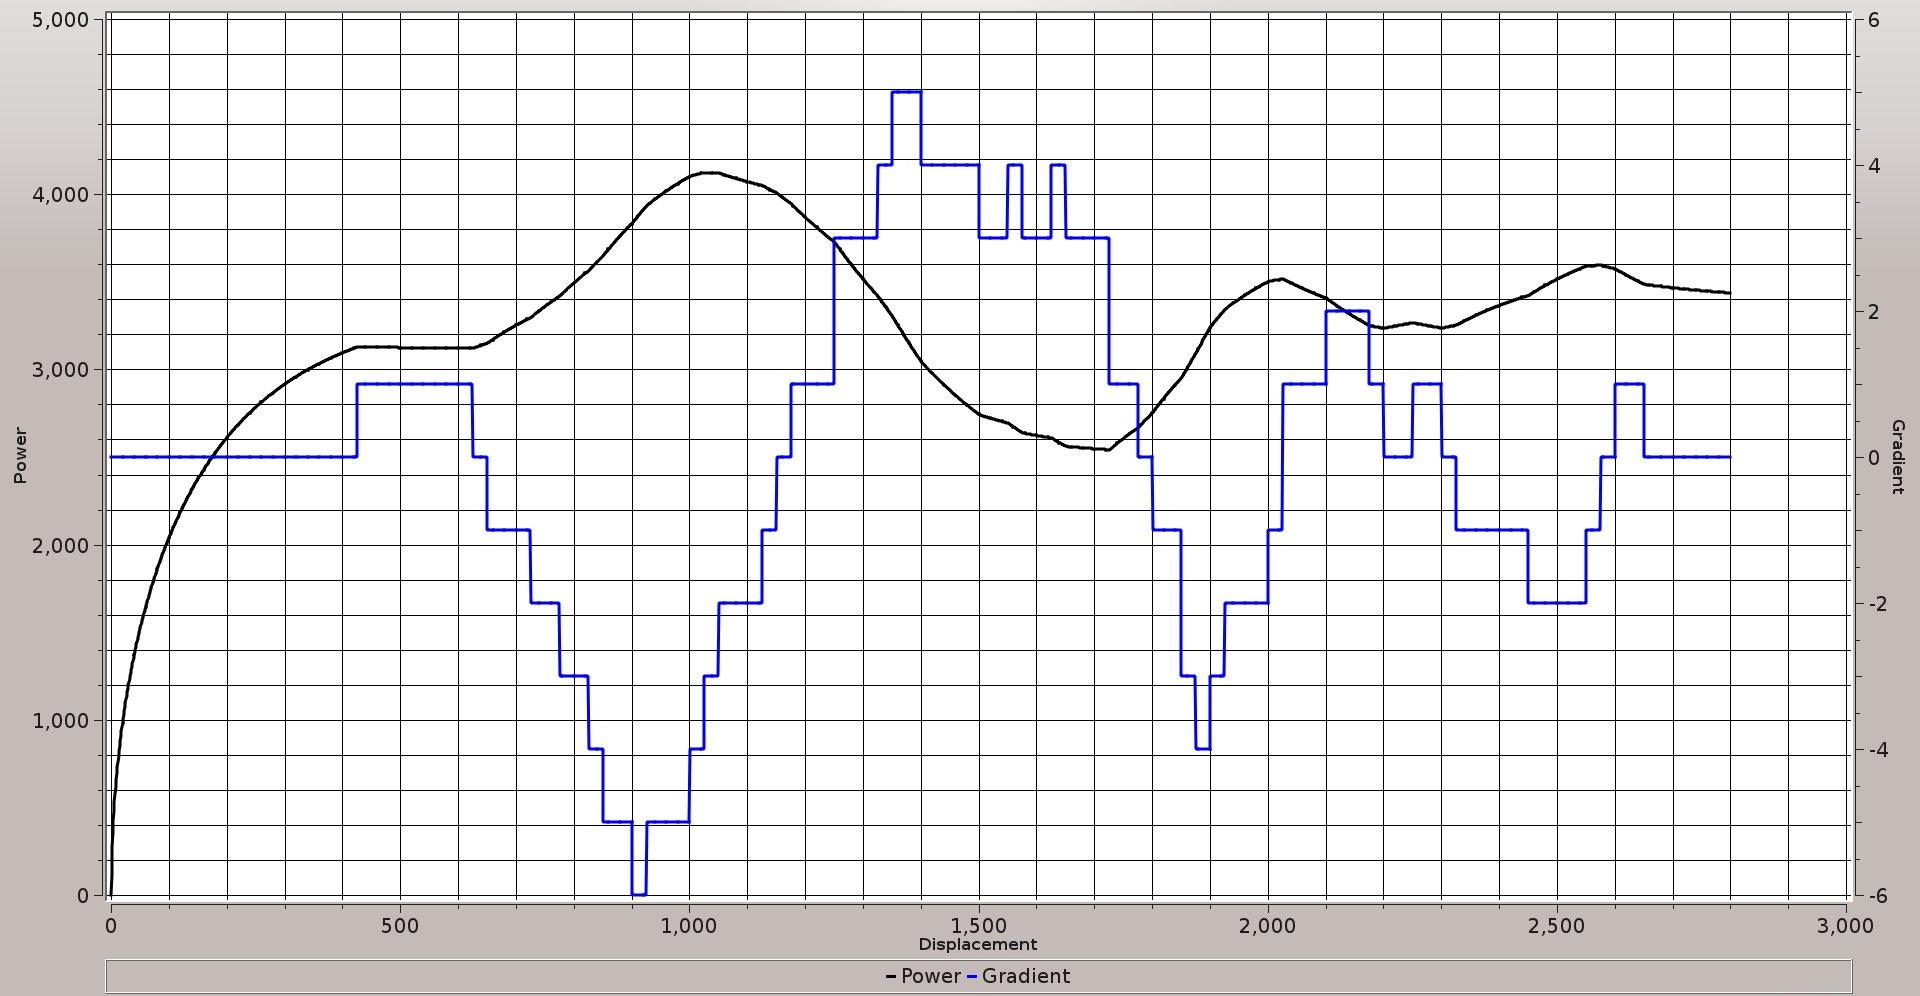
\includegraphics[width=6in]{images/0_2.jpg}
	\caption{Graph of power and gradient versus displacement for "full throttle everywhere"}
	\label{im:0_2}
\end{figure}

Figure \ref{im:0_3} displays the graph of air drag versus displacement. Again, the air-drag profile is similar to the vehicle speed curve because the air-drag force is proportional to the square of the velocity of the vehicle. The maximum air drag occurs when the speed of the vehicle hits maximum with the magnitude of 120 N.m of torque needed for overcoming the air-drag.

\begin{figure}[htb]
	\centering
	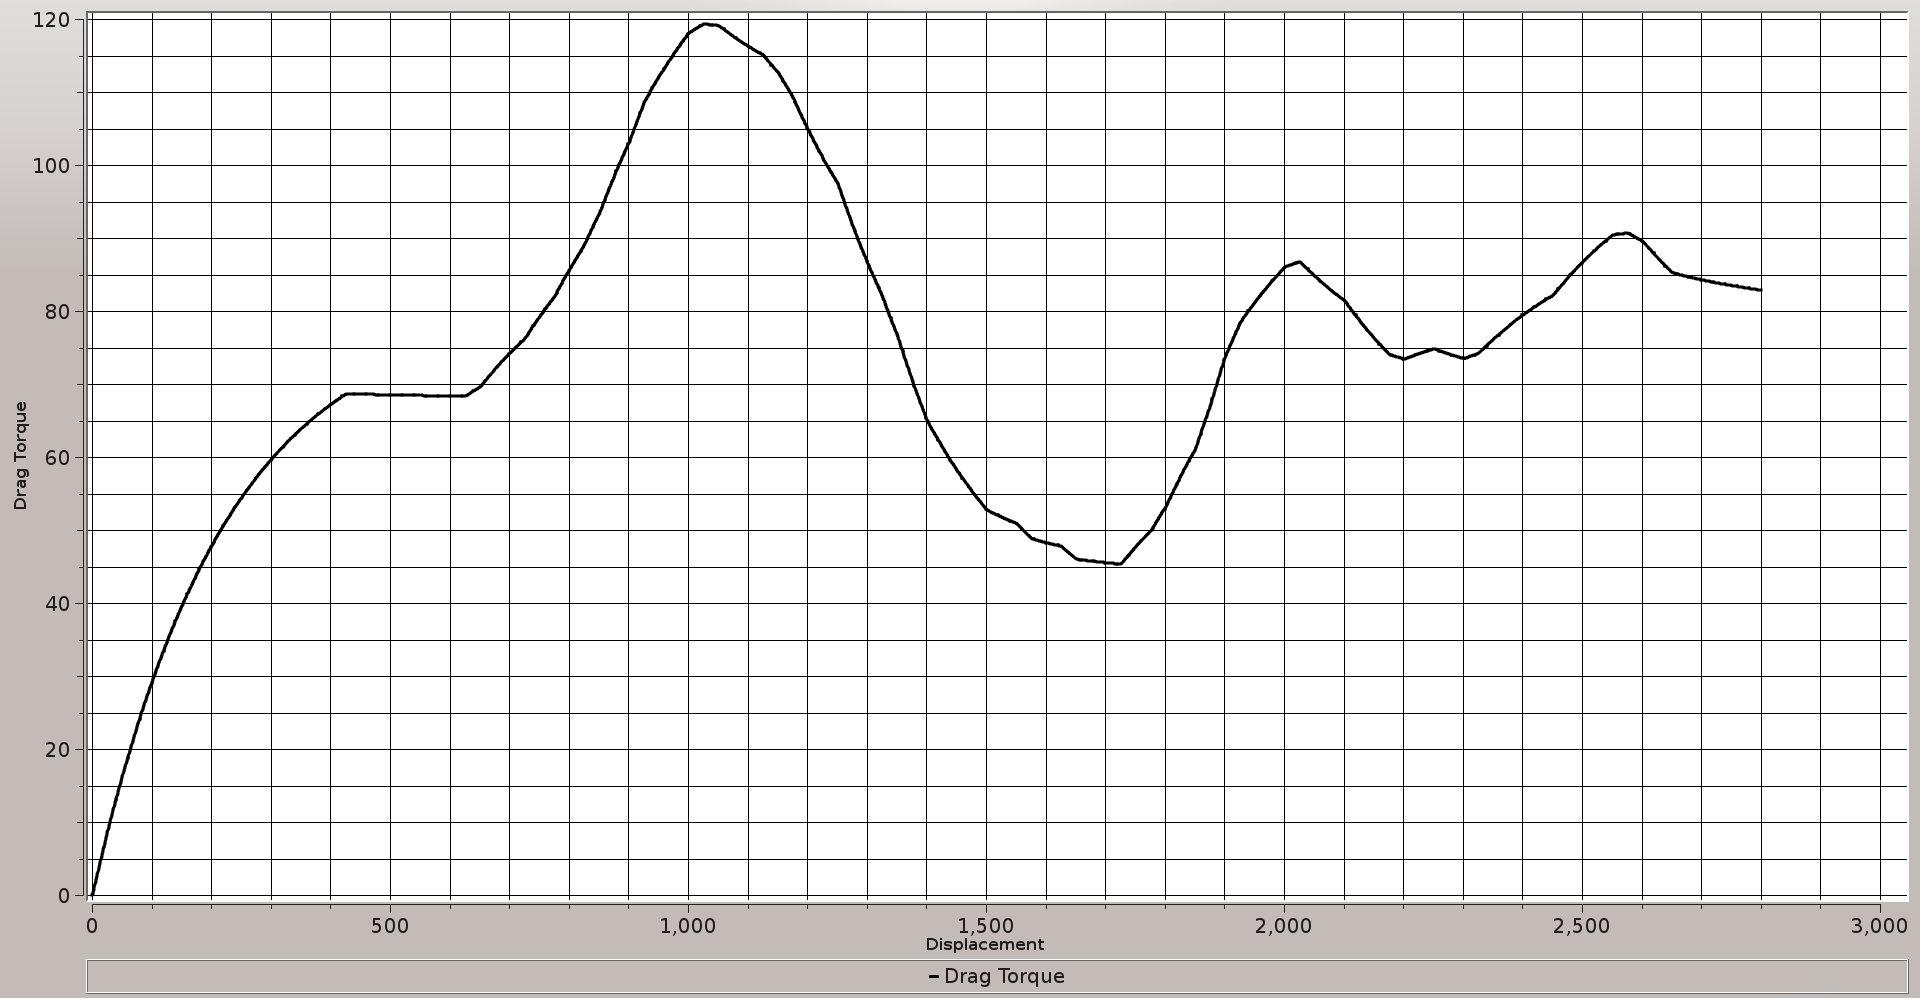
\includegraphics[width=6in]{images/0_3.jpg}
	\caption{Graph of air drag versus displacement for "full throttle everywhere"}
	\label{im:0_3}
\end{figure}

Table \ref{tb:fullThrottleResult} shows the main result for the "Full Throttle Everywhere". As shown in the table, the total energy consumption as simulated is 560003J and the lap time is 187 seconds. The total time for 4 laps will be 748 seconds, with 10 seconds of stops between each lap and some time wasted, the time for completion for 1 attempt will be 788 seconds which is 13 minutes and 8 seconds. The mileage calculated from the energy consumption is 18 km/kWh. 

\begin{table}[htbp]
\begin{center}
\begin{tabular}{|c|c|}
\hline
\textbf{Result} & \textbf{Value} \\ \hline
Total Energy Consumption & 560003J \\ \hline
Total Time for 1 Lap & 186.981s \\ \hline
Mileage & 18 km/kWh \\ \hline
\end{tabular}
\end{center}
\caption{Main result for "Full Throttle Everywhere" }
\label{tb:fullThrottleResult}
\end{table} \clearpage

\section{Strategies}
There are 3 strategies composed for improving the mileage of the electric vehicle on the Sepang North Track.

\subsection{Preset Strategy 1}

The "Full Throttle Everywhere" strategy listed at the previous section is not effective because the torque generated by the electric motor is excessive at most of the part of the circuit. Therefore, a better strategy is produced which is the "Preset Strategy 1". The "Preset Strategy 1" reduces the energy consumption of the electric vehicle by turning off the electric motor so that the electric vehicle cruise down the hill when the gradient is less than 0\textdegree \ . By using the simulation software, the result of "Preset Strategy 1" is shown at the following graphs.

Figure \ref{im:1_1} shows the graph of speed and gradient versus displacement for "Preset Strategy 1". The speed profile of the electric vehicle shown in this graph is different with the speed curve in figure \ref{im:0_1} since the vehicle is set to cruise when the gradient is negative. The maximum speed of the vehicle is less than the maximum speed for "FUll Throttle Everywhere" strategy which has a value of 15.7m/s and happens at the end of starting straight. The speed of the vehicle drops gradually when going downhill because the gravitational force is insufficient for countering the rolling resistance and air drag. The vehicle pick up speed when the gradient of the track is less than 3\textdegree and started to slow down when the gradient is higher due to the inadequate torque generated by the electric motor.

\begin{figure}[htb]
	\centering
	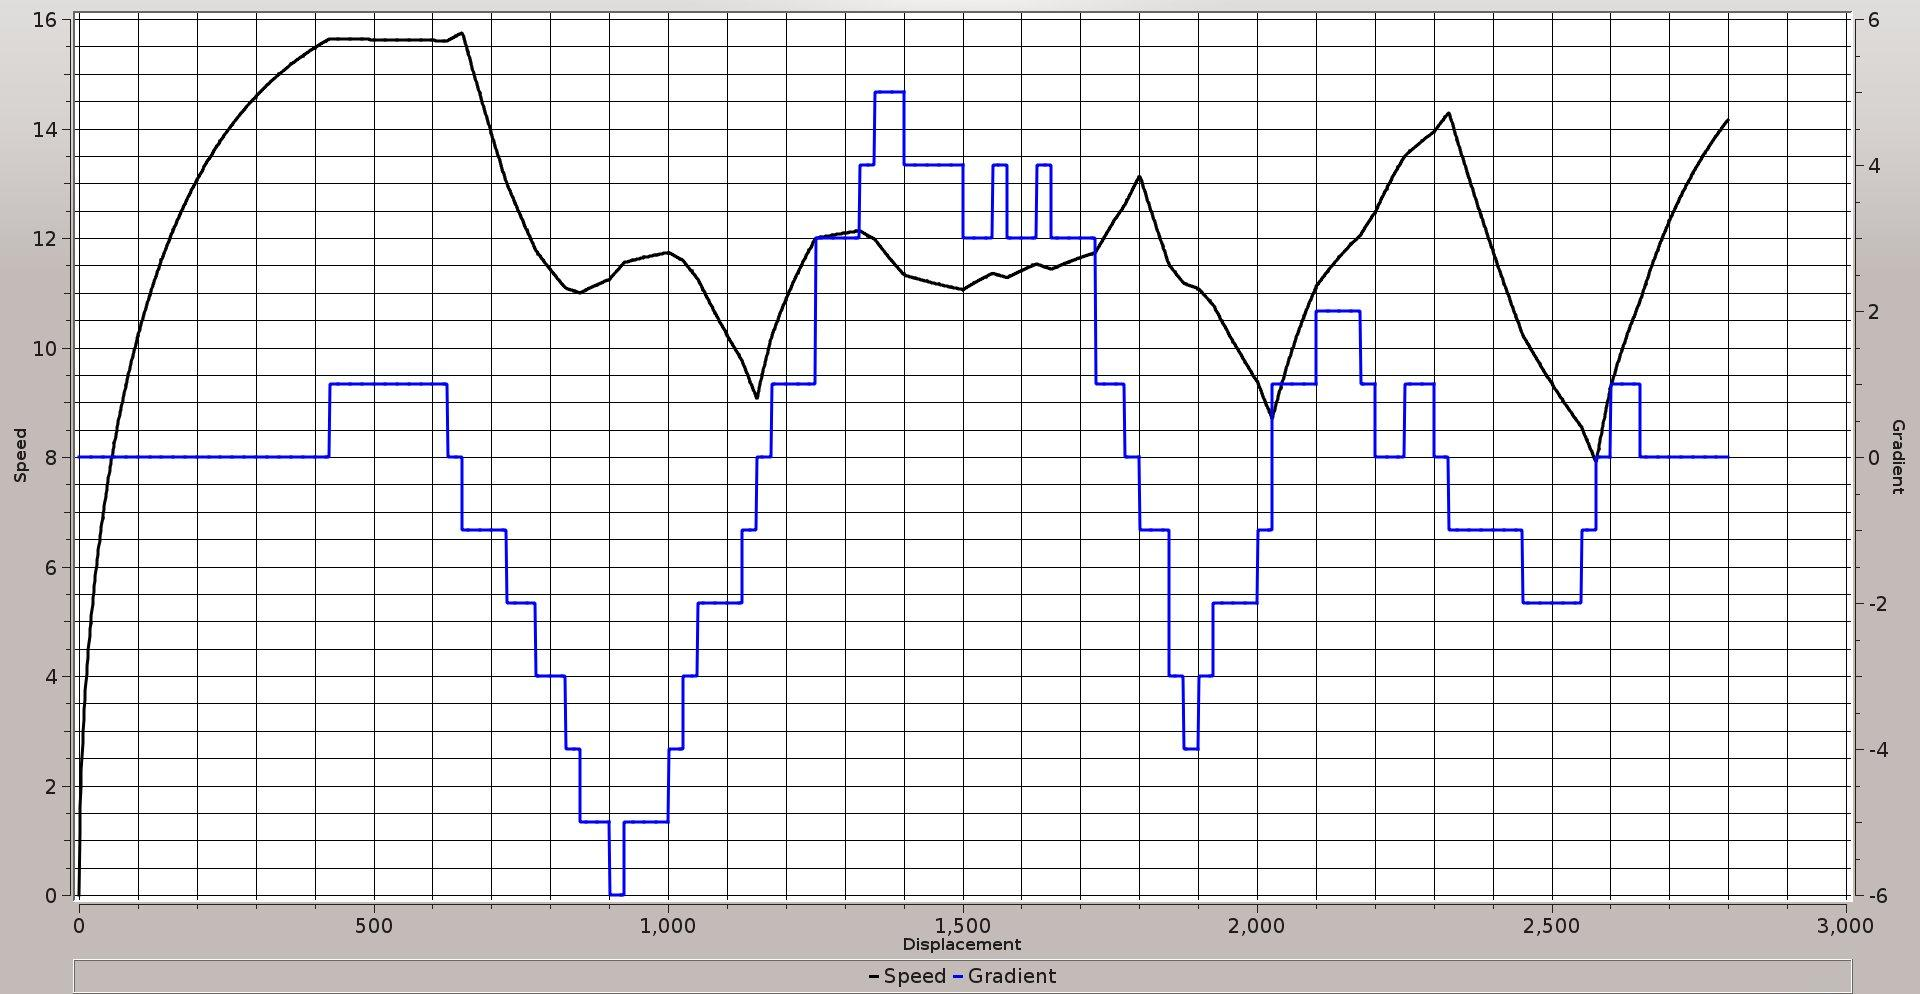
\includegraphics[width=6in]{images/1_1.jpg}
	\caption{Graph of Speed and Gradient versus displacement for "Preset Strategy 1"}
	\label{im:1_1}
\end{figure}

Figure \ref{im:1_2} shows the graph of power and gradient versus the displacement for "Preset Strategy 1". The power curve shows a huge rise at the beginning straight. The power output of the electric vehicle is 0 when cruising down and the power output surge again when the vehicle is driving on the flat road or up the hill. Since the speed of the vehicle is less than the speed of the vehicle in "Full Throttle Everywhere" strategy, the maximum output also drops from over 4kW for the previous strategy to around 3.1kW for the current strategy.

\begin{figure}[htb]
	\centering
	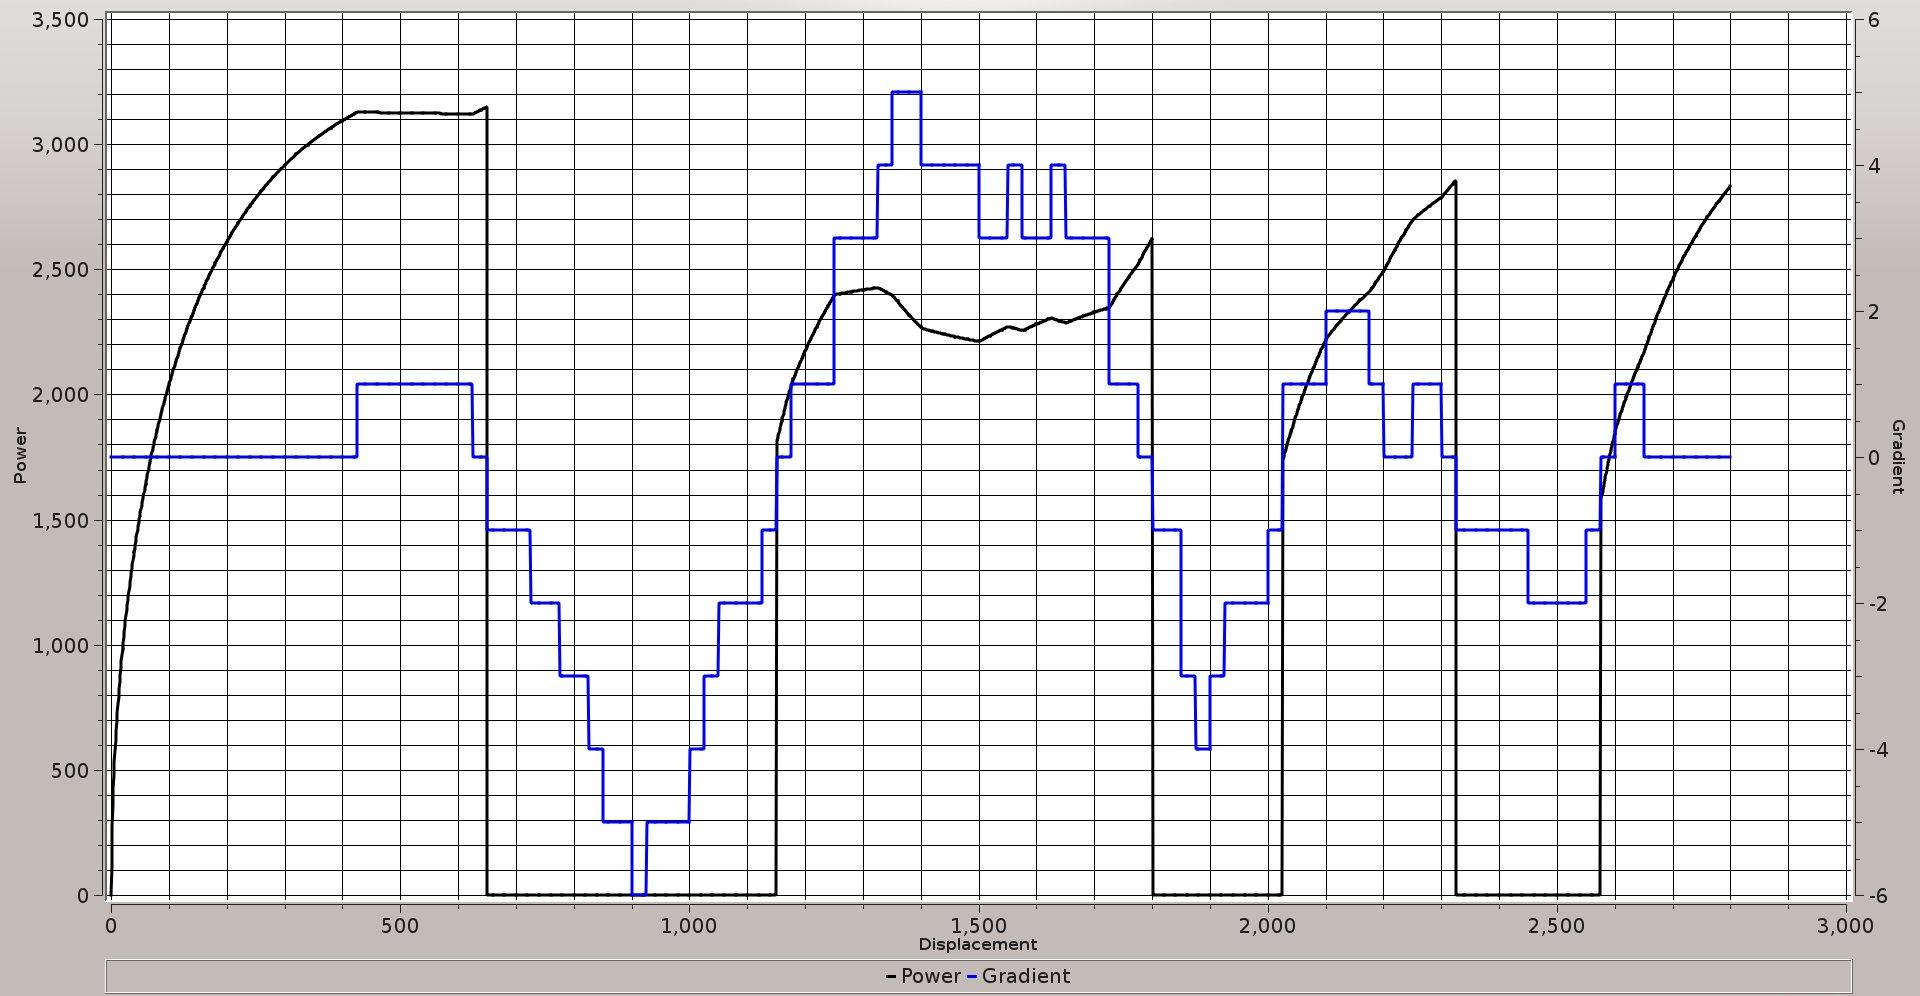
\includegraphics[width=6in]{images/1_2.jpg}
	\caption{Graph of Power and Gradient versus displacement for "Preset Strategy 1"}
	\label{im:1_2}
\end{figure}

Since the maximum vehicle speed is reduced by 23.8\% , the maximum torque need to be supplied by the electric motor for counter air drag force reduces from 120 N.m to 69.5 N.m, which is a huge 42\% improvement as shown in figure \ref{im:1_3}.

\begin{figure}[htb]
	\centering
	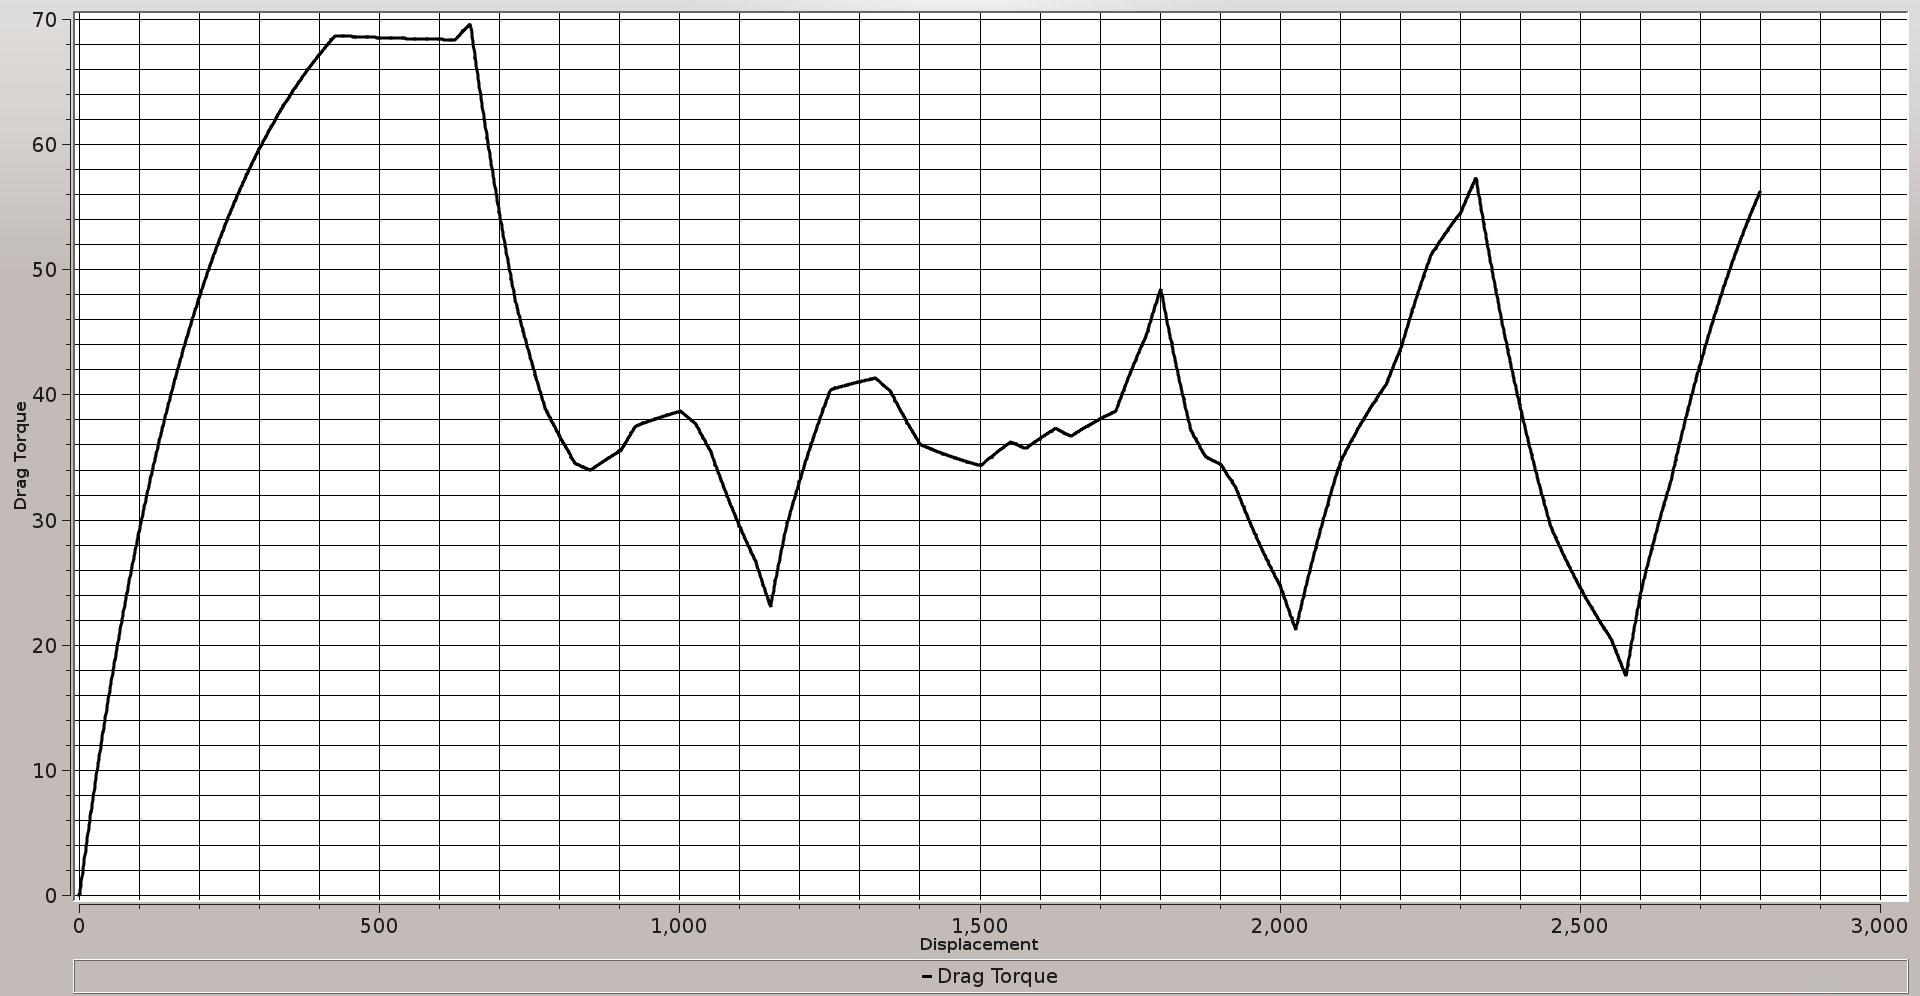
\includegraphics[width=6in]{images/1_3.jpg}
	\caption{Graph of air drag versus displacement for "Preset Strategy 1"}
	\label{im:1_3}
\end{figure}

Table \ref{tb:preset1Result} shows the overall result simulated using "Preset Strategy 1". The total energy consumption is reduced to 365004J but the lap time is increased to 247 seconds. The time for 1 attempt is increases to 1026 seconds which is 17 minutes and 6 seconds which is within the time limit. The mileage using Preset Strategy 1 is improved to 27.6 km/KWh.

\begin{table}[htbp]
\begin{center}
\begin{tabular}{|c|c|}
\hline
\textbf{Result} & \textbf{Value} \\ \hline
Total Energy Consumption & 365004J \\ \hline
Total Time for 1 Lap & 246.554s \\ \hline
Mileage & 27.6 km/kWh \\ \hline
\end{tabular}
\end{center}
\caption{Main result for "Preset Strategy 1" }
\label{tb:preset1Result}
\end{table} \clearpage

\subsection{Preset Strategy 2}
Since the "Preset Strategy 1" waste a lot of energy by accelerating through the ending straight and the speed of the vehicle is stil reducable for reducing the effect of air-drag, "Preset Strategy 2" is set so that the vehicle cruise to the end of a lap and the speed is controlled within 14m/s and the vehicle started to cruise at 2650m displacement onwards until the start/finish line.

Figure \ref{im:2_1} shows the graph of speed and gradient versus displacement. The speed curve is similar to the speed curve for "Preset Strategy 1" except that the top speed of the electric vehicle is limited to 14m/s by the strategy. The curve after 2650 displacement is also dropping which is different than previus strategy. 

\begin{figure}[htb]
	\centering
	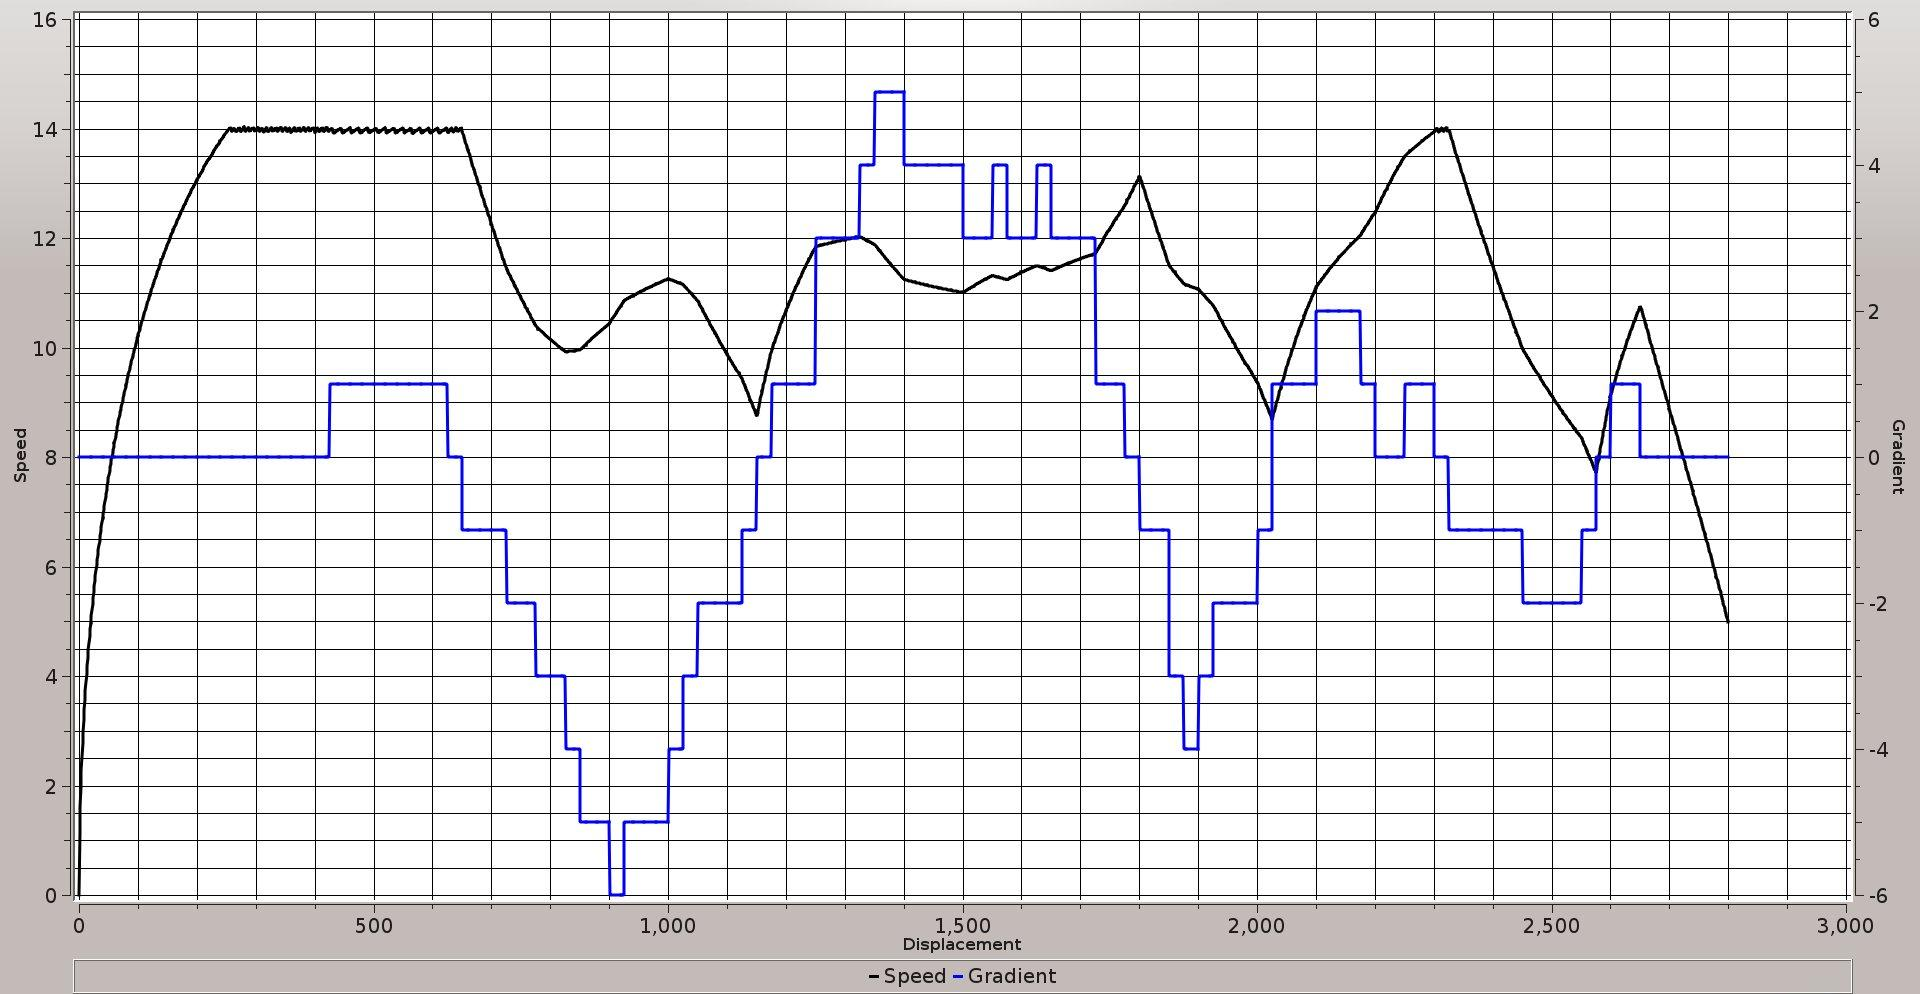
\includegraphics[width=6in]{images/2_1.jpg}
	\caption{Graph of Speed and Gradient versus displacement for "Preset Strategy 2"}
	\label{im:2_1}
\end{figure}

Figure \ref{im:2_2} is the graph of power and gradient versus displacement. The power curve is similar to the power curve for the previous strategy with some minor difference which is the power output of the electric motor is 0 near the end of the circuit (after 2650m). In addition, lot's of fluctuation is observed between 250m to 650m displacement. This is because the simulation set the throttle to 0 and 1 alternatively for maintaining the top speed at 14m/s which is similar to the principle of PWM. In real life, switching between minimum and maximum throttle frequently will create lot's of current spike and hence waste more energy. Therefore, in actual race, the driver have to adjust the throttle so that the speed maintain at 14m/s. 

\begin{figure}[htb]
	\centering
	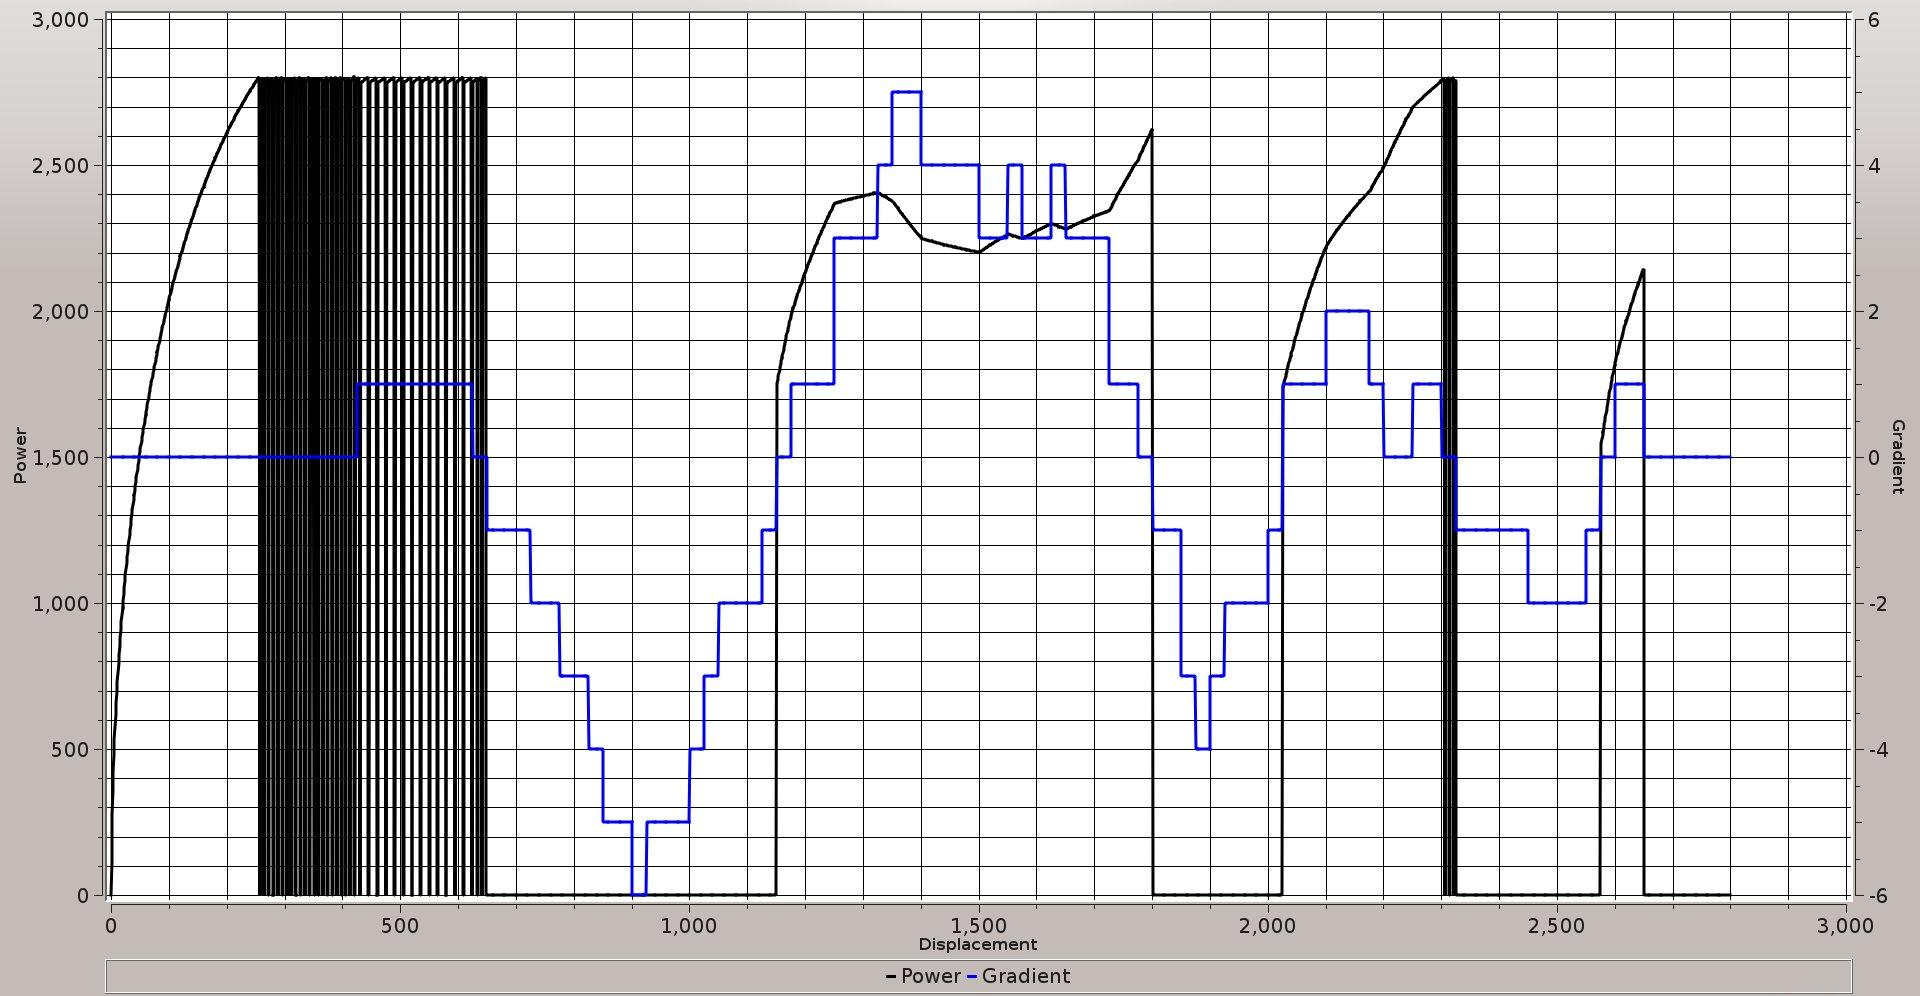
\includegraphics[width=6in]{images/2_2.jpg}
	\caption{Graph of Power and Gradient versus displacement for "Preset Strategy 2"}
	\label{im:2_2}
\end{figure}

Figure \ref{im:2_3} shows the air drag versus the displacement for "Preset Strategy 2". As the maximum speed is limited to 14m/s, the maximum torque needed by the electric motor for countering the air drag drops to 52.5N.m which is another 24.5\% improvement over the previous strategy.

\begin{figure}[htb]
	\centering
	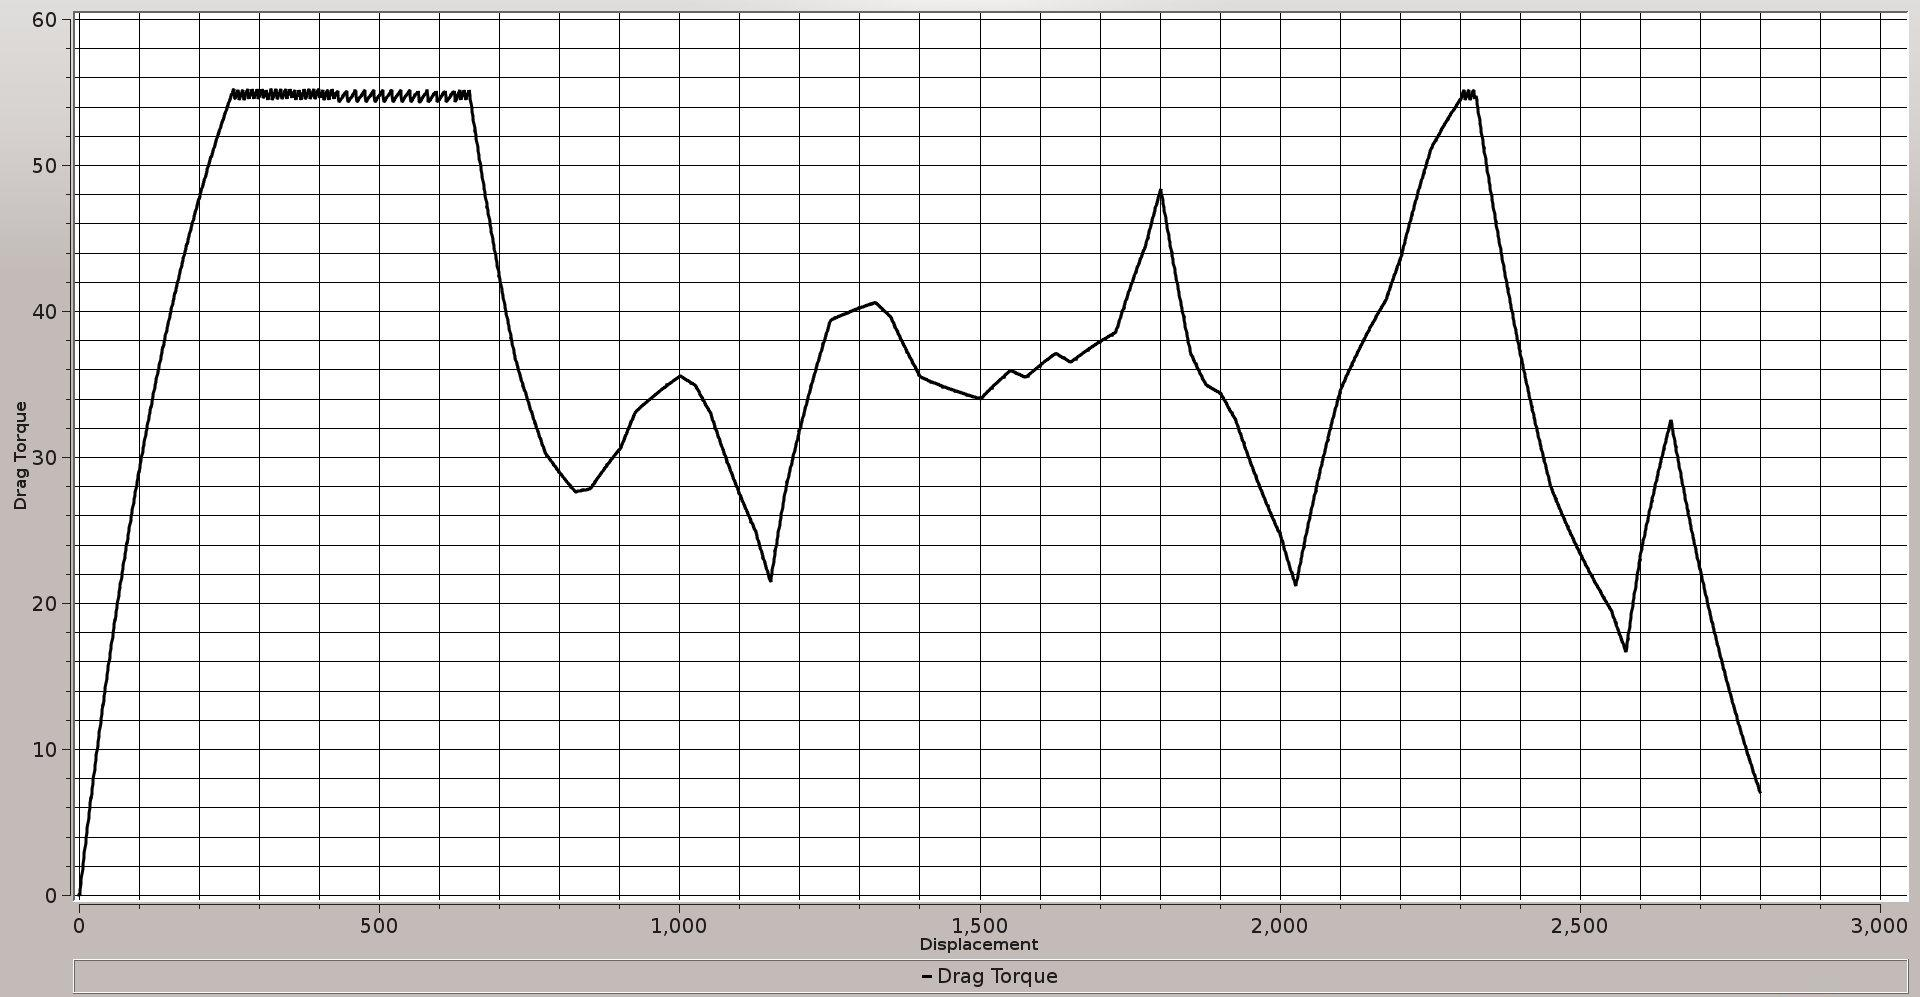
\includegraphics[width=6in]{images/2_3.jpg}
	\caption{Graph of air drag versus displacement for "Preset Strategy 2"}
	\label{im:2_3}
\end{figure}

Table \ref{tb:preset2Result} shows the main result for "Preset Strategy 2". As shown in the tablem the energy consumption is reduced to 318200J hence the mileage increases to 31.7km/kWh. Due to the top speed limitation, the average speed of the vehicle reduces. Therefore the lap time increases to 262 seconds yielding the total time for 1 attempt to be 1087 seconds which is 18 minutes 7 seconds. 

\begin{table}[htbp]
\begin{center}
\begin{tabular}{|c|c|}
\hline
\textbf{Result} & \textbf{Value} \\ \hline
Total Energy Consumption & 318200J \\ \hline
Total Time for 1 Lap & 261.699s \\ \hline
Mileage & 31.7 km/kWh \\ \hline
\end{tabular}
\end{center}
\caption{Main result for "Preset Strategy 2" }
\label{tb:preset2Result}
\end{table} \clearpage

\subsection{Preset Strategy 3}

"Preset Strategy 2" reduces the energy consumption of the electric vehicle compared to "Preset Strategy 1" but there is still room of improvement because full throttle is aplied when the vehicle is climbing so the generated torque at some section may exceed the required torque which will then accelerate the vehicle when driving uphill. Therefore, a new strategy is composed to tackle this problem which is the "Preset Strategy 3".

The "Preset Strategy 3" is a strategy which has the following characteristics:

\begin{itemize}
	\item{Gradual acceleration, limit the acceleration to 0.13m/$s^2$.}
	\item{The speed is limited to 11m/s-12m/s at flat road before 2600m displacement.}
	\item{Vehicle cruising after 2600m displacement.}
	\item{Vehicle maintain at constant speed when driving up the slope.}
	\item{Vehicle cruising when driving down the slope.}
\end{itemize}

Figure \ref{im:3_1} shows the speed and gradient versus the displacement graph. From the graph, the maximum speed of the electric vehicle is reduced to 11.9m/s. The speed when the vehicle is driving up the hill is almost constant with low magnitude fluctuation due to the calculation of air drag using the previous velocity. 

\begin{figure}[htb]
	\centering
	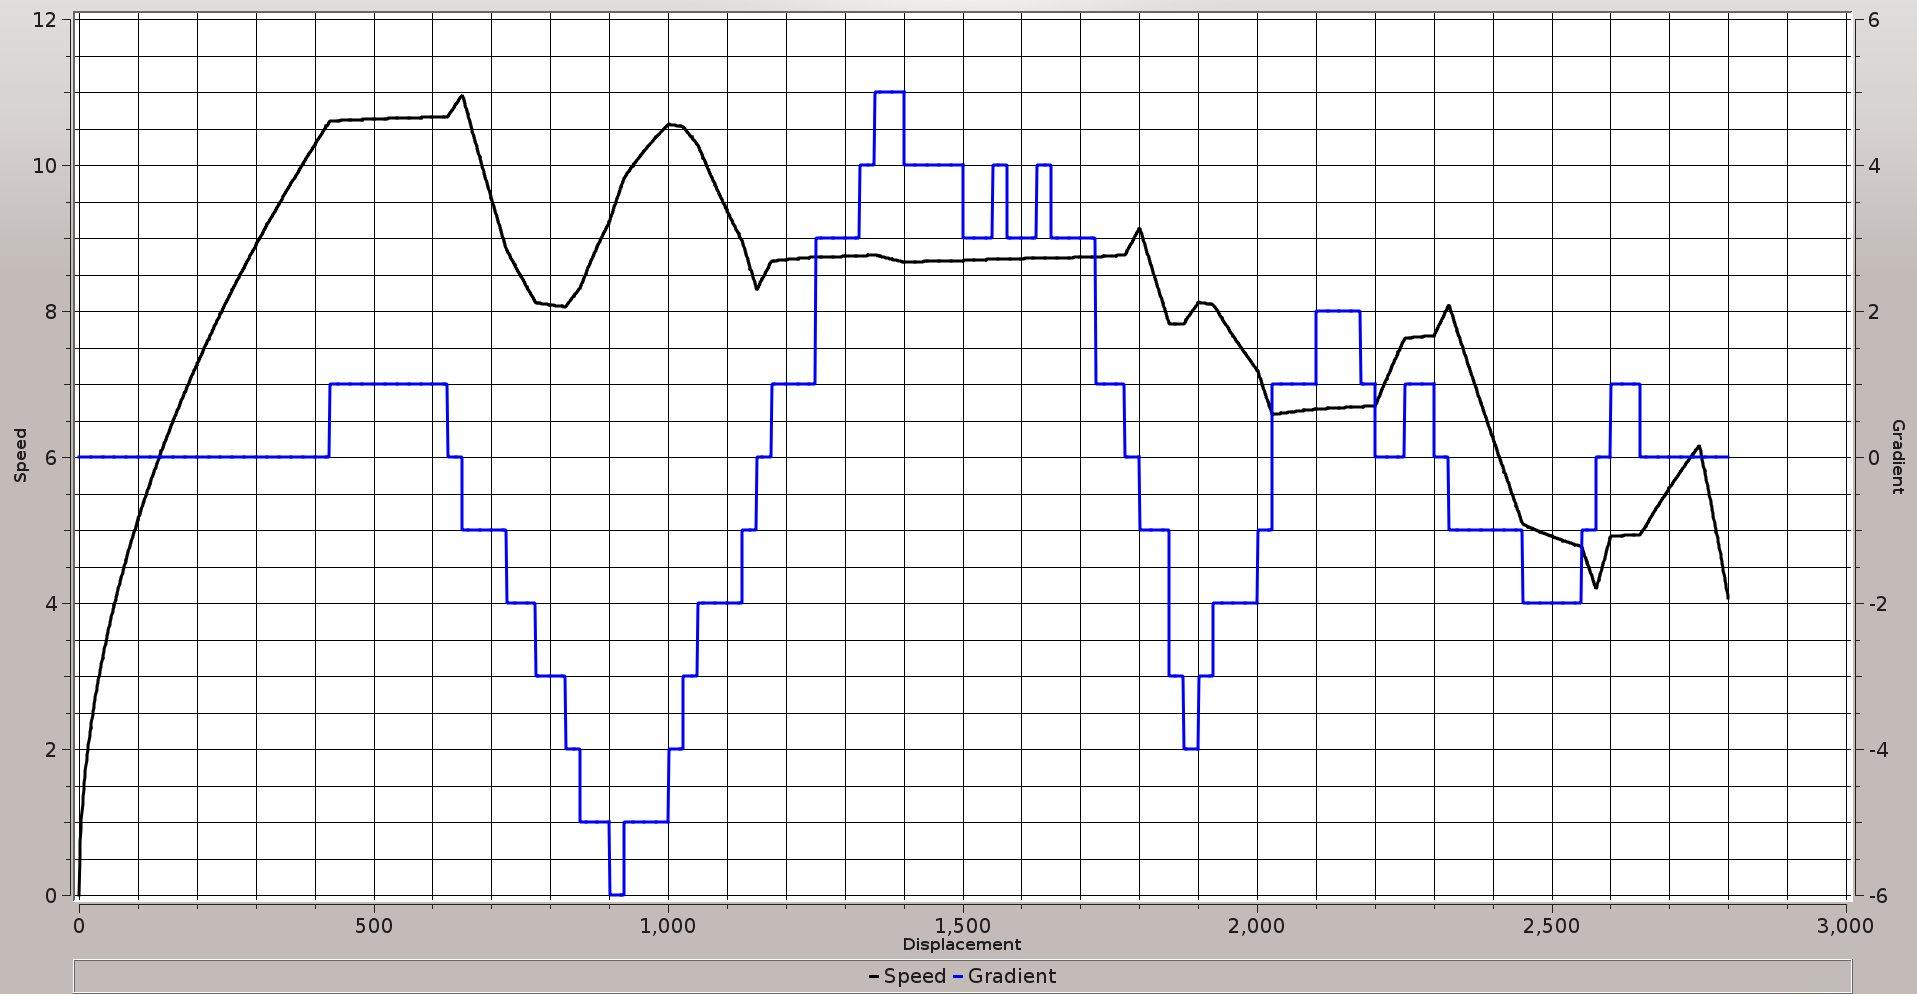
\includegraphics[width=6in]{images/3_1.jpg}
	\caption{Graph of Speed and Gradient versus displacement for "Preset Strategy 3"}
	\label{im:3_1}
\end{figure}

Figure \ref{im:3_2} shows the power and gradient versus displacement graph. As shown in the graph, the power output of the electric vehicle matches the gradient of the track with some minor offset contributed by the acceleration of the vehicle and the air drag on the vehicle. The maximum power output power occurs at around 1350m displacement with a value of 1.75kW. 

\begin{figure}[htb]
	\centering
	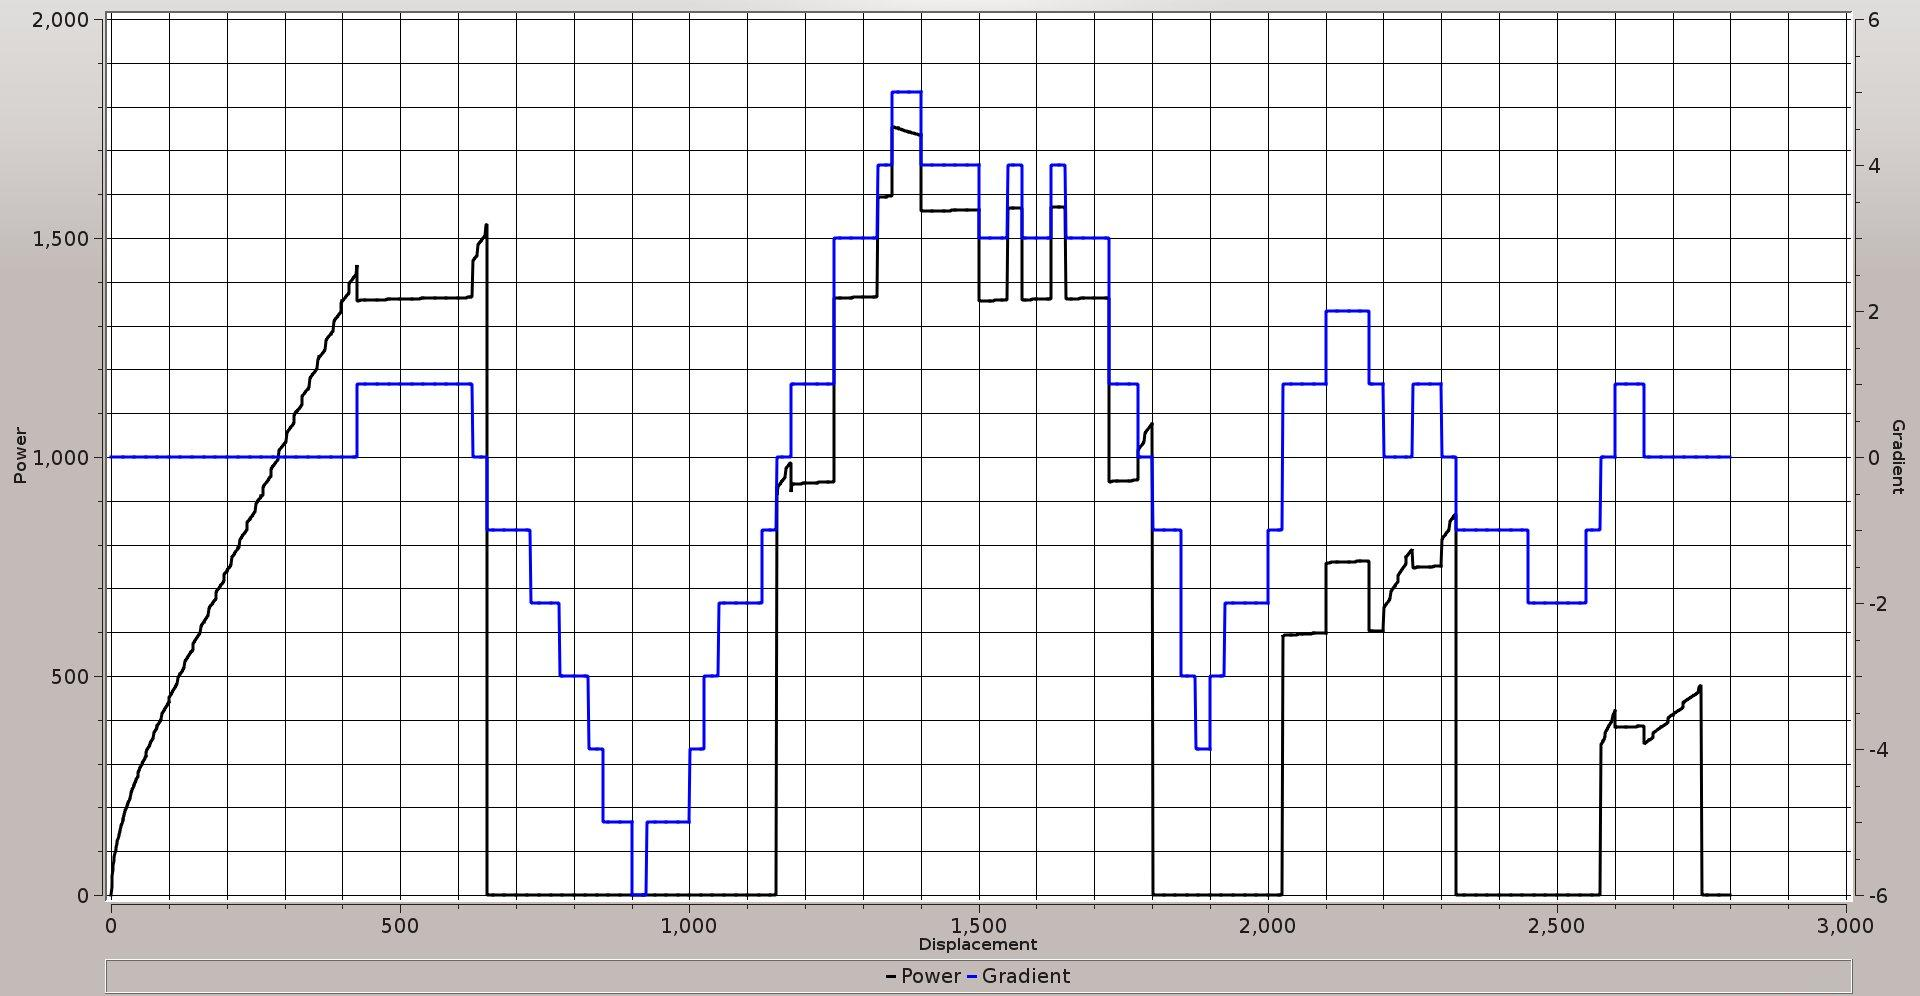
\includegraphics[width=6in]{images/3_2.jpg}
	\caption{Graph of Power and Gradient versus displacement for "Preset Strategy 3"}
	\label{im:3_2}
\end{figure}

Figure \ref{im:3_3} shows the graph of air drag versus displacement for "Preset Strategy 3". Again, the maximum torque required to overcome the air drag reduced from previous strategies' value to 34N.m which occurs at around 650m displacement due to the peak vehicle speed at that point. By implementing this strategy, the maximum air drag dropped by 35.2\% .

\begin{figure}[htb]
	\centering
	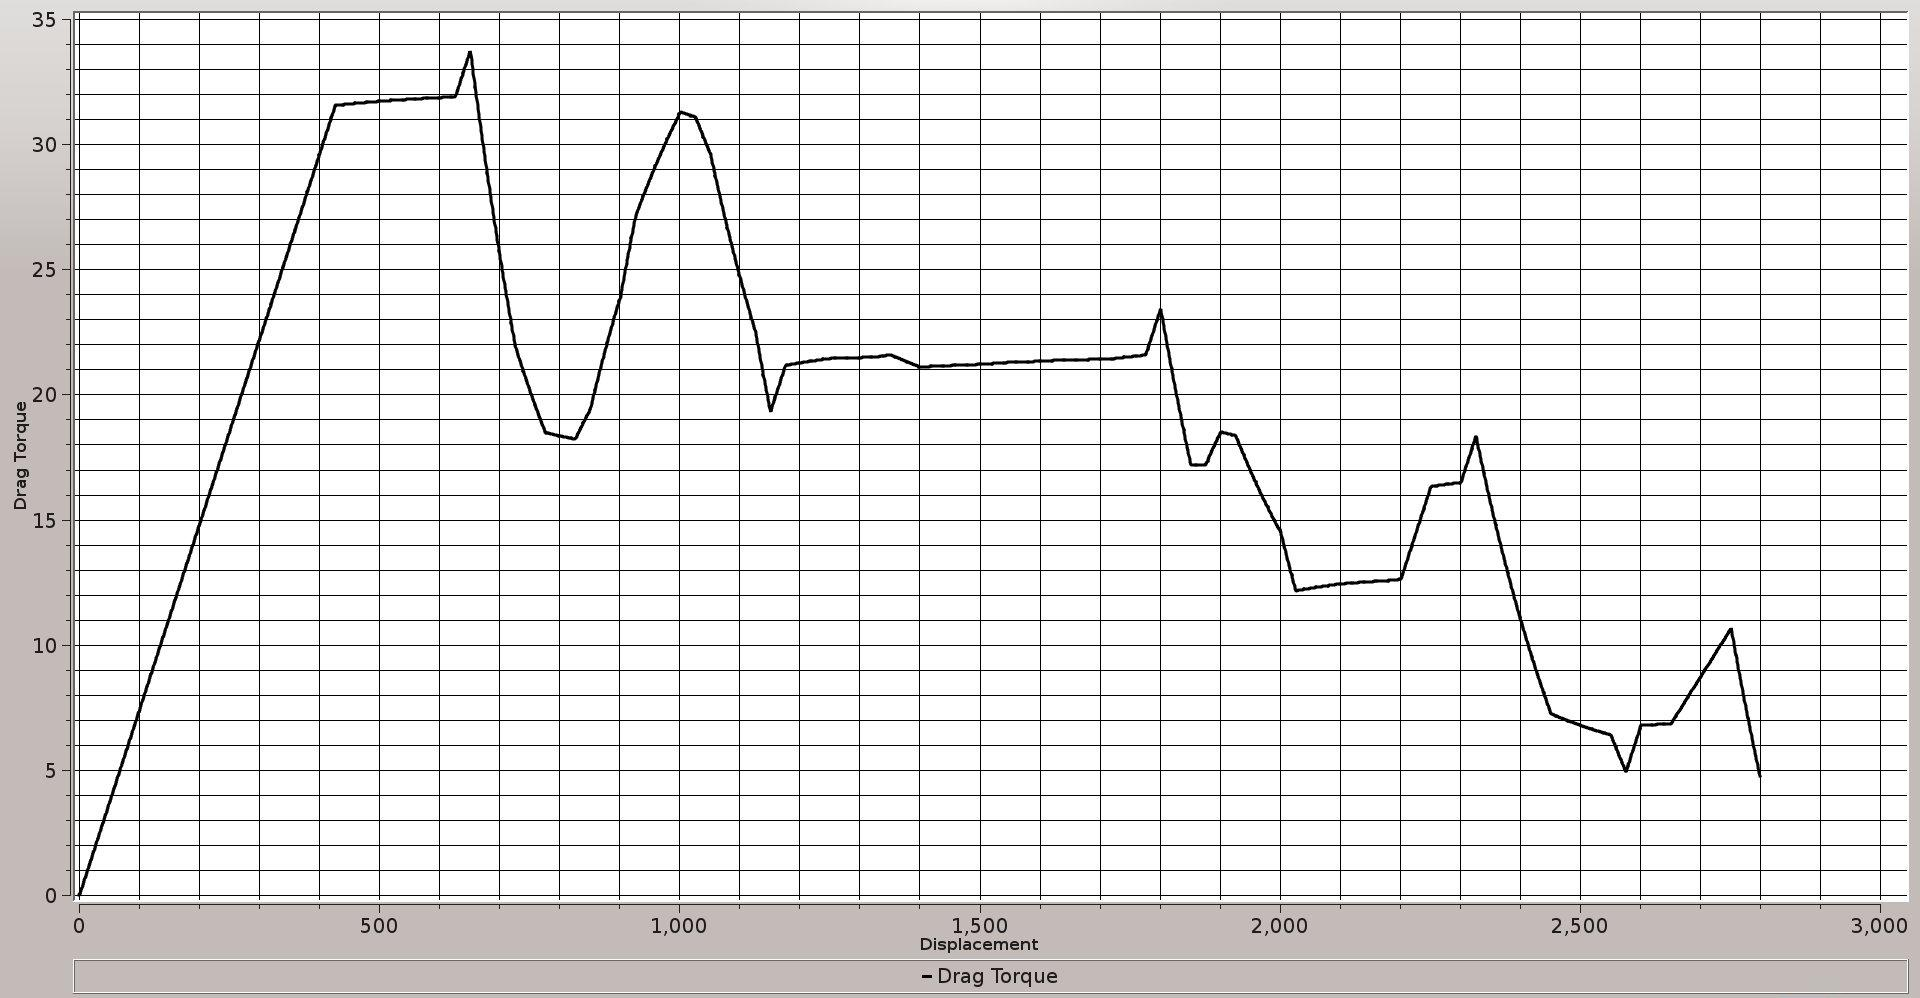
\includegraphics[width=6in]{images/3_3.jpg}
	\caption{Graph of air drag versus displacement for "Preset Strategy 3"}
	\label{im:3_3}
\end{figure}

Table \ref{tb:preset3Result} shows the main simulation result for "Preset Strategy 3". The total energy consumption is less than the previous strategies which is 216385J and the mileage increases to 46.6km/kWh. The lap time is increases to 390.491 seconds, hence the attempt time would be 1602 seconds which is equal to 26 mins and 42 seconds. The attempt time is slightly (1 minute and 18 seconds) under the time limit (28 minutes).

\begin{table}[htbp]
\begin{center}
\begin{tabular}{|c|c|}
\hline
\textbf{Result} & \textbf{Value} \\ \hline
Total Energy Consumption & 216385J \\ \hline
Total Time for 1 Lap & 390.491s \\ \hline
Mileage & 46.6 km/kWh \\ \hline
\end{tabular}
\end{center}
\caption{Main result for "Preset Strategy 3" }
\label{tb:preset3Result}
\end{table} \clearpage

\subsection{Comparison Between Preset Strategies}
\section{Summary}
